% remember to set these at the start of each chapter
\chapter{Experiments and Discussion} 

%%%%%%%%%%%%%%%%%%
\section{Dataset}
The dataset is obtained from western university. It contains 90 specimen samples, each of which has an Ultrasound (US) image stack and a Photoacoustic (PAT) image stack. The type of cancer (class) of each specimen is given in the dataset. The distribution of classes is 
{'B': 33, 'C': 21, 'A': 8, 'F': 6, 'E': 5, 'G': 5, 'H': 2, 'I': 2, 'K': 2, 'D': 1, 'L': 1, 'N': 1, 'J': 1, 'M': 1}.  
In this project, only class B and C are used. B has 33 samples and C has 21 samples. The other classes have too few samples to train a neural network on. 

For each image stack, US and PAT, the centre few images are extracted to use for training and testing. In a top-down scan of a specimen, the centre few images usually have the most detail and thus have most information of the specimen which work the best in classifying the specimen. An example of image stack is shown in Fig.\,\ref{stack}.

\begin{figure}[h]
	\centering
	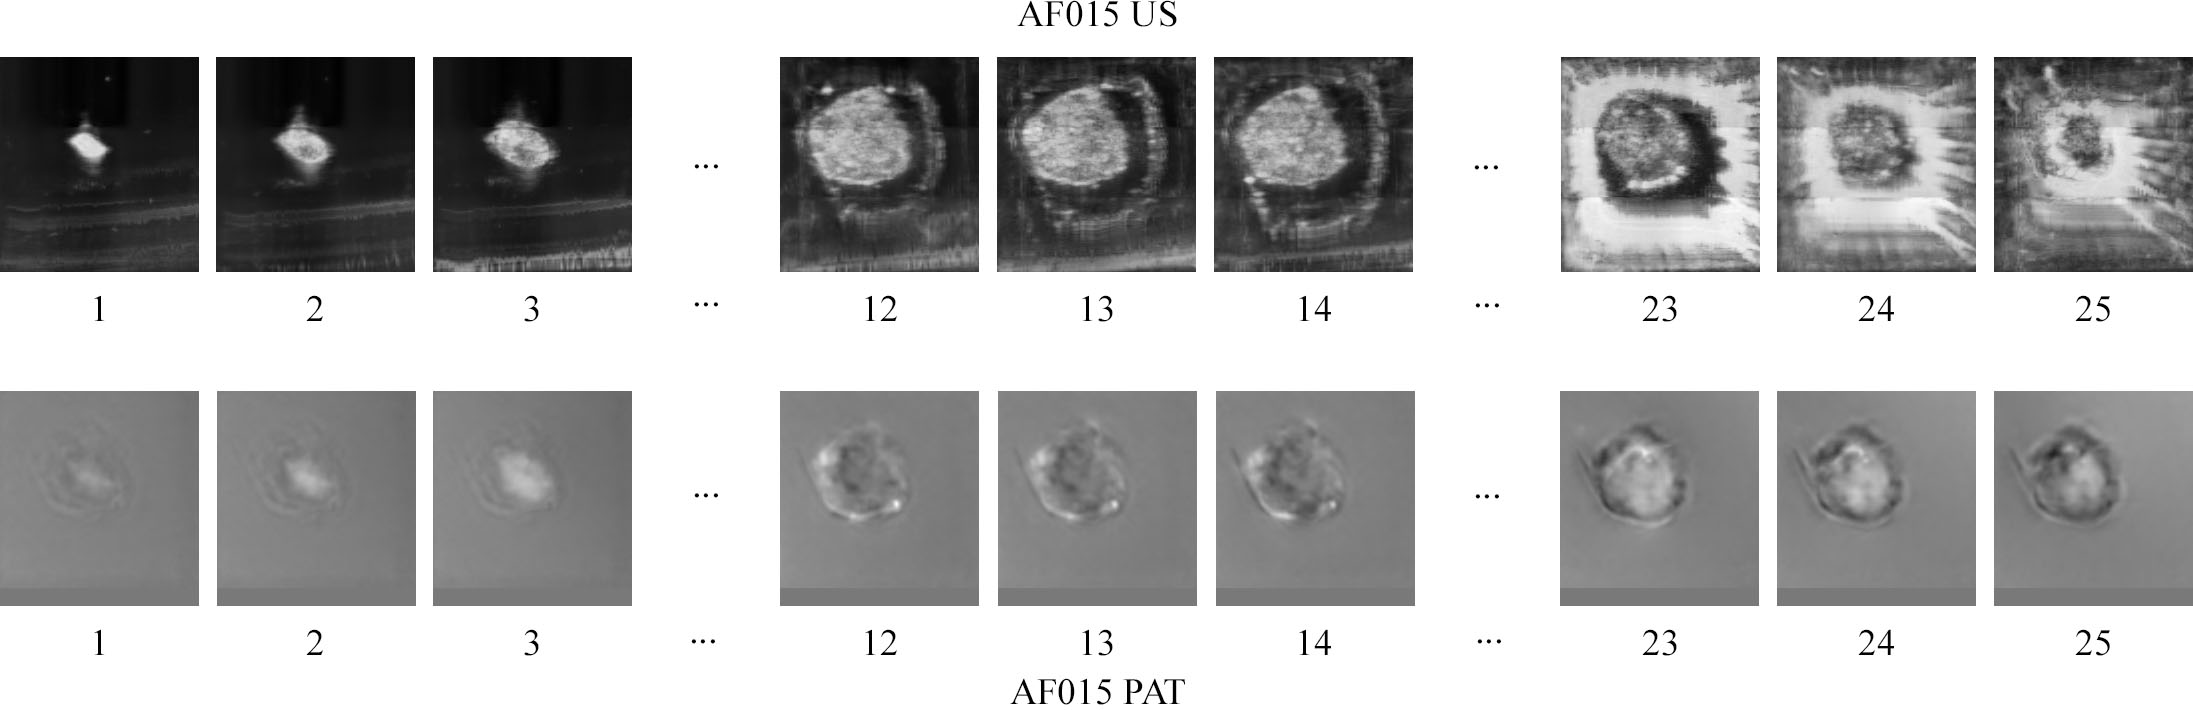
\includegraphics[width=\textwidth]{Figs/stack.jpg}
    \caption{US PAT stack example}
    \label{stack}
\end{figure}

We can see that the top few and bottom few scans have very low quality and lack of detail of the internal texture. The scans close to centre are larger in size and have the texture that classification could depend on.


\section{Data Partition and Augmentation}
The specimen samples are divided into training set and testing set by 0.8 ratio, 5-fold cross validation is used. Centre 6 images are extracted from a stack. No images from the same stack is separated into training and testing set. The images are resized to (200,200).

Machine learning requires large amounts of data. While our dataset is very small, data augmentation is used to artificially expanding the number of samples. Augmentation Scaling Factor is set to 5, meaning five images are created from one by Rotation, Cropping, Horizontal and Vertical Flip.

\section{Training}
"Adam" optimizer is used in all models to minimize the categorical cross-entropy across two classes. Adam is a replacement optimization algorithm for classic stochastic gradient descent. Adam can adaptively adjust the parameter learning rates based on the average first moment (the mean), as well as the average of the second moments of the gradients (the uncentered variance). The parameters of Adam optimizer is set to default. All samples are passed to the network 50 times, with a batch size of 64. Best set of weights is saved. All parameters can be modified in YAML format for easier parameter fine tuning.


\section{Training Curves}

From the training curves, we can see that all training loss is decreasing and accuracy is increasing.

Unrepresentative Train Dataset
An unrepresentative training dataset means that the training dataset does not provide sufficient information to learn the problem, relative to the validation dataset used to evaluate it.
This may occur if the training dataset has too few examples as compared to the validation dataset.
This situation can be identified by a learning curve for training loss that shows improvement and similarly a learning curve for validation loss that shows improvement, but a large gap remains between both curves.
Unrepresentative Validation Dataset
An unrepresentative validation dataset means that the validation dataset does not provide sufficient information to evaluate the ability of the model to generalize.
This may occur if the validation dataset has too few examples as compared to the training dataset.
This case can be identified by a learning curve for training loss that looks like a good fit (or other fits) and a learning curve for validation loss that shows noisy movements around the training loss.


\section{$F_1$ score}
The $F_1$ score (also F-score) is a measure of a test's accuracy. It considers both the precision $p$ and the recall $r$ of the test to compute the score: $p$ is the number of correct positive results divided by the number of all positive results returned by the classifier, and $r$ is the number of correct positive results divided by the number of all relevant samples (all samples that should have been identified as positive). The $F_1$ score is the harmonic average of the precision and recall, where an $F_1$ score reaches its best value at 1 (perfect precision and recall) and worst at 0.
Formally $F_1$ score = $2 \cdot \frac{precision \cdot recall}{precision + recall}$.
presition $p = \frac{TP}{TP + FP}$
recall $r = \frac{TP}{TP + FN}$
true positives (TP): Samples which we predicted belong to a class, and they are indeed in the class.
true negatives (TN): Samples which we predicted not belong to a class, and they are indeed not in that class.
false positives (FP): We predicted in a class, but they are actually not.
false negatives (FN): We predicted not in a class, but they are actually in.
